\section{Introducci\'on}
El problema para este ejercicio es el siguiente, se nos presentan $n$ productos qu\'imicos, los cuales deben transportarse en camiones de un lugar a otro, el llevar al elemento $i$ en el mismo cami\'on que otro elemento $j$, conlleva una ''peligrosidad'' asociada $h_i_j$. El objetivo del algoritmo ser\'a encontrar la soluci\'on que utilize la menor cantidad de cami\'ones posibles, pero que cada cami\'on tenga una peligrosidad menor a una cota $m$.
\\
La entrada del problema consiste en:
\\
\begin{itemize}
\item Un entero \textbf{n} $\rightarrow$ Representar\'an el n\'umero de productos qu\'imicos a transportar.
\item Un entero \textbf{m} $\rightarrow$ Representar\'a la cota de peligrosidad que ningun cami\'on puede superar.
\item \textbf{n-1} filas donde, para cada fila $i$ consta de $n-i$ enteros:
\begin{itemize}
\item $h_i_{,i+1}, h_i_{,i+2}$ ... $h_i_{,n}$ $\rightarrow$ Representar\'an la peligrosidad asociada del elemento $i$ con los elementos $i+1$, $i+2$ ... $n$.
\end{itemize}
\end{itemize}
\\
La salida, por su parte, constar\'a de una fila con:
\\
\begin{itemize}
\item Un entero \textbf{C} $\rightarrow$ Representar\'a la cantidad indispensable de cami\'ones que es necesaria para transportar los productos bajo las condiciones del problema.
\item $n$ enteros $\rightarrow$ Representar\'an en que cami\'on viaja cada producto.
\end{itemize}

\subsection{Ejemplo de entrada valida}
Hagamos un peque�o ejemplo para que pueda ilustrarse bien el problema.
\\
Supongamos que tenemos $3$ productos qu\'imicos, el producto $1$ es muy inestable, por lo que si es transportado con el producto $2$ la peligrosidad asociada al camion en el que viajan estos dos productos asciende a $40$, y si se transporta con el producto $3$ la peligrosidad ser\'a de $35$. El producto $2$ en cambio es de naturaleza mas estable, por lo que si es transportado con el producto $3$ solo produce una peligrosidad de $3$.
\\
Por otro lado queremos que la peligrosidad por cami\'on no supere el valor de $39$.
\\
Entonces la entrada para este problema ser\'a:
\\
\\
$\textbf{3 39}$
\\
$\textbf{40 35}$
\\
$\textbf{3}$
\\
\\
Para una entrada de estas dimenciones es posible buscar la mejor solucio\'on a mano.
\\
Las posibles combinaciones son que los tres productos viajen juntos, que los tres viajen separados en camiones distintos, que $1$ y $2$ viajen juntos en el mismo camion y el producto $3$ viaje en otro cami\'on diferente, que $1$ y $3$ viajen juntos y el $2$ separado y que $2$ y $3$ viajen juntos y el producto sobrante viaje en otro cami\'on.
\\
La primera d\'a una peligrosidad de $40+35+3$ por lo la cota de peligrosidad se ve superada, lo que lo vuelve una soluci\'on inviable, la segunda es valida, ya que la peligrosidad de cada camion es $0$, pero se necesitan $3$ camiones. Que $1$ y $2$ viajen juntos, tampoco es valida, la peligrosidad de ese camion es demaciado alta, y finalmente las ultimas dos son validas (peligrosidad $35$ y $3$, respectivamente) y solo son necesarios dos camiones.
\\
Es claro, luego, que las dos ultimas soluciones son las que el algoritmo podr\'ia devolever.
\\
Luego las dos salidas que podr\'a devolver el algoritmo son:
\begin{itemize}
\item $2$ $1$ $2$ $1$
\end{itemize}
o
\begin{itemize}
\item $2$ $1$ $2$ $2$
\end{itemize}
\\
\section{Idea General de Resoluci\'on}
Luego la idea del algoritmo es simple, probar todas las combinaciones posibles de camiones y de entre todas determinar cual es la que cumple con la cota de peligrosidad pedida y usa la menor cantidad de camiones posible. Ademas, para aumentar la performance del algoritmo, se ir\'an podando ramas de la familia de soluciones de manera tal de que no sea necesario chequear absolutamente todos los casos.
\\
Antes de presentar el pseudocodigo vale aclarar un punto importante y es que el algoritmo debe encontar siempre una soluci\'on. Esto se debe a que siempre es posible poner todos los productos qu\'imicos en camiones separados, lo que nos d\'a  una peligrosidad $0$. Es posible usar esta como una cota contra la cual parar de chequear, si tenemos $n$ productos qu\'imicos, es simple ver que a lo sumo usar\'emos $n$ camiones. Denominaremos a esta como la "peor soluci\'on" ya que es claro que es una soluci\'on valida, pero que usa la maxima cantidad de camiones.
\\
En cuanto a las podas, utilizamos dos, una que en cada paso del backtrack chequea si la soluci\'on final que encontramos hasta el momento usa una cantidad menor de camiones que la solucion parcial que se esta construyendo. Es claro que de ser as\'i, estamos la solucion parcial nunca podr\'a ser mejor, por lo tanto se podar\'a toda esa familia de soluciones.
\\
La segunda chequea que la soluci\'on parcial que estamos construyendo no exceda el limite de peligrosidad pedido por el ejercicio, en caso de ser as\'i la soluci\'on no ser\'a valida. En caso de que esto suceda, tambien se poda.
\\
Finalmente el pseudocodigo para resolver este problema queda as\'i:

\begin{algorithm}
\begin{algorithmic}[1]\parskip=1mm
\caption{void FuncionPrincipal()}

  \STATE{Generar una matriz con las peligrosidades entre los distintos productos}
  
  \STATE{Se inicializa la solucion final, como la peor de las soluciones}
  
  \STATE{Backtrack(tablaDePeligrosidad, solucionParcial, solucionFinal)}
  
  \STATE{Mostar la soluci\'on final}
 
 \end{algorithmic}
\end{algorithm}

\begin{algorithm}
\begin{algorithmic}[1]\parskip=1mm
\caption{Bool Backtrack(tablaDePeligrosidad, solucionParcial, solucioninal)}
	
	\STATE{Llamo a la funcion check(tablaDePeligrosidad, solucionParcial, solucionFinal)}
	
	\STATE{\quad Si check devuelve $2$, la solucion parcial es mejor que la final}
	\STATE{\quad \quad Pongo la solucion parcial como final} 
	\STATE{\quad \quad Corto la recursi\'on y busco por otra rama}

	\STATE{\quad Si check devuelve $0$, la cota de peligrosidad fu\'e sobrepasada}
	\STATE{\quad \quad esta rama no me sirve, podo}	

	\STATE{\quad Si check devuelve $3$, la solucion anterior usa menos camiones}
	\STATE{\quad \quad esta rama no me sirve, podo}

	\STATE{\quad Si check devuelve $1$, la solucion es valida, pero no est\'a completa}
	\STATE{\quad \quad contin\'uo agregando camiones}

	\STATE{Para cada valor $i$ de $1$ hasta $n$ prueba meter el siguiente producto de la lista en el camion $i$ y se llama a la funcion Backtrack()}
\end{algorithmic}
\end{algorithm}

\begin{algorithm}
\begin{algorithmic}[1]\parskip=1mm
\caption{int check(tablaDePeligrosidad, solucionParcial, solucionFinal)}


	\STATE{Checkeo si la solucion final usa menos camiones ~~~~~~~~~~~~ $O(n)$}
	\STATE{\quad Si es verdad}
	\STATE{\quad \quad Devuelvo $3$}


	\STATE{Checkeo si la cota de peligrosidad fue sobrepasada ~~~~~~~~~~~~ $O(n^2)$}
	\STATE{\quad Si es verdad}
	\STATE{\quad \quad Devuelvo $0$}


	\STATE{Checkeo si la cada producto tiene un camion asignado ~~~~~~~~~~~~ $O(1)$}
	\STATE{\quad Si es verdad}
	\STATE{\quad \quad Devuelvo $2$}

\STATE{Devuelvo $1$}

\end{algorithmic}
\end{algorithm}

\newpage
\section{Correctitud}
Seg\'un lo desarrollado en la idea principal, sabemos que el algoritmo siempre tend\'a una soluci\'on y esta se encuentra acotada en un vector de $n$ elementos cada uno entre $1$ y $n$. Dado que el rango es acotado, un algoritmo que chequee todas las posibles soluciones y devuelva la soluci\'on valida que usa menos camiones, ser\'a un algoritmo correcto.
\\
Ahora lo que resta demostrar es que las podas que realizamos, no quitan soluciones v\'alidas.
\\
La primera de las podas chequea que si la soluci\'on parcial excede la cota $m$. Es claro ver que cualquier soluci\'on que tenga una sub-soluci\'on inv\'alida nunca podr\'a ser v\'alida, por lo tanto se puede descartar sin necesidad de completarla.
\\
La segunda de las podas chequea que la soluci\'on que estamos construyendo tenga menos camiones que la mejor soluci\'on que tenemos hasta el momento. Esto es, si s\'e que puedo llevar los $n$ productos qu\'imicos en $j$ camiones, no es necesario explorar las soluciones que contengan m\'as de $j$ camiones, estas soluciones jam\'as podr\'an ser mejores que la soluci\'on que ya tengo.
\\
Luego quitando esa parte del espacio de soluci\'ones no estoy quitando en ningun momento posibles soluciones \'optimas, ergo, el algoritmo es correcto.  
\\
\section{Complejidad}
Por cada producto qu\'imico, el algoritmo de backtrack intenta ponerlo en cualquiera de los $n$ posibles camiones, y realiza $O(n^2)$ chequeos intentando podar.
\\
Entonces la formula quedar\'a:
\\
$$T(i) = T(i-1)n + n^2$$
\\
$$T(1) = n + n^2$$
\\
Luego para el peor de los casos el algoritmo tendr\'a una complejidad de $O(n^n)$.
\\
\section{Resultados}
\subsection{Testing}

\subsection{Caso Random}
Para testear la performance de nuestro algoritmo se cre\'o un generador de entradas que fabricar\'a instancias random del problema. Luego se comparar\'a el tiempo que tarda nuestro algoritmo contra uno que encuentre la soluci\'on utilizando fuerza bruta y tambi\'en contra otro backtracking, pero con las podas invertidas, o sea primero chequea si la cantidad de camiones de la soluci\'on parcial es menor a la cantidad de camiones de la mejor soluci\'on hasta el momento y luego chequea que la cota de peligrosidad sea la correcta, para ver si esto var\'ia de alguna manera la complejidad.
\\
El testeo consisti\'o en generar 40 instancias del problema para cada $n$ diferente, con un $m$ fijo y valores de peligrosidad entre productos qu\'imicos que var\'ian entre $1$ y $m$. Luego se tom\'o la media y compararon los resultados:
\\
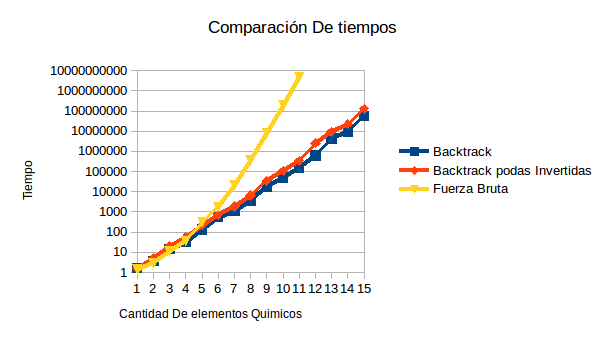
\includegraphics[width=18cm]{./Ej3/graph1.png}
\\
En el gr\'afico puede verse que nuestro algoritmo es notablemente superior a un algoritmo de fuerza bruta, ya que escala mucho mejor con respecto a $n$ y levemente mejor al backtracking con las podas invertidas. Para los casos de $14$ y $15$ elementos el backtracking pudo arrojar una respuesta en un tiempo admisible, mientras que el de fuerza bruta ya tardaba tiempos completamente fuera de escala.
\\
Para comprobar de manera experimental que la complejidad del algoritmo solo depende de $n$ tambi\'en se realiz\'o lo mismo variando la cota de peligrosidad $m$, para un $n$ fijo igual a $9$.
\\
Los resultados arrojados pueden verse en el siguiente gr\'afico:
\\
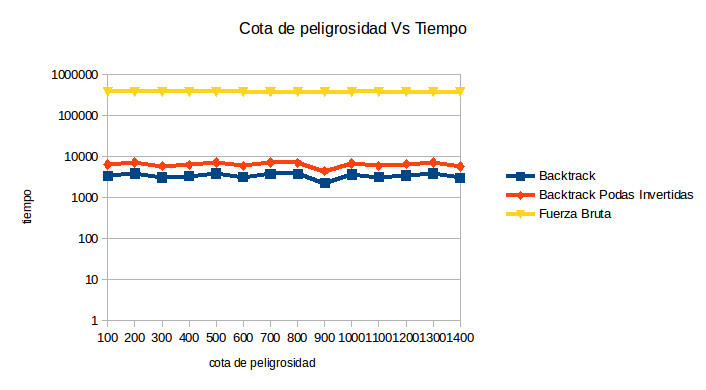
\includegraphics[width=18cm]{./Ej3/graph2.png}
\\
Luego es claro que ninguno de los algoritmos depende de $m$. Adem\'as en este gr\'afico puede volverse a apreciar de manera visible la mejora de nuestro algoritmo con respecto a uno de fuerza bruta.
\\
\subsection{Peor caso}
Otro test que podemos intentar realizar es ver si nuestro algoritmo presenta alguna mejora al de fuerza bruta en el peor de los casos, esto es, en el caso de que cada producto tenga que viajar forzosamente en un cami\'on diferente, obligando de cierta manera a nuestro algoritmo a chequear todos los reslutados posibles, sin poder realizar podas significativas.
\\
Para testear esto tomamos nuevamente $40$ muestras aleatorias, con un $m$ fijo en $10$, valores de peligrosidad los productos entre $m$ y $m+2$ las corremos en los tres algoritmos.
\\
Los resultados pueden verse en el siguiente cuadro:
\\
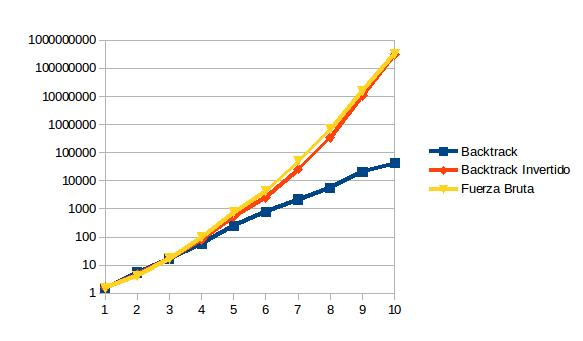
\includegraphics[width=18cm]{./Ej3/peorGraph.jpg}
\\
Puede verse aqu\'i que nuestra soluci\'on contin\'ua siendo mejor que uno de fuerza bruta. En este caso, el otro backtracking con las podas invertidas muestra una notable perdida de performance, siendo casi tan malo como el algoritmo de fuerza bruta.
